\documentclass[]{article}
\usepackage[a4paper, margin=0.5in]{geometry}
\usepackage{graphicx}
\usepackage{listings}
\usepackage{xcolor}

\title{\textbf{The Word Ladder Problem }\\ Artificial Intelligence}
\author{Suhas N (EC21B1113), Reddappa Reddy (EC21B1114)}

\lstset{language=Python,
	basicstyle=\small\ttffont,
	keywordstyle=\color{blue},
	commentstyle=\color{gray},
	stringstyle=\color{green},
	numbers=left,
	numberstyle=\small,
	numbersep=5pt,
	breaklines=true,
	tabsize=4,
	frame=single}

\begin{document}

\maketitle

\section{Introduction}

The Word Ladder Problem is a puzzle in which the objective is to transform one word into another by changing a single letter at a time, with the constraint that each intermediate step must also be a valid word. The challenge is to find the shortest sequence of such transformations, known as the word ladder, linking the initial word to the target word. The Word Ladder Problem has applications in various fields, including natural language processing, search engines, and puzzle-solving algorithms.

\section{Solving the Problem}

\subsection{Gathering the data}

To solve the word ladder problem, we need to form a corpus of words. We have taken the words from the following sources:

\begin{itemize}
	\item Books listed on Project Gutenberg (https://www.gutenberg.org/)
	\item The Wordnet database (from python-nltk)
\end{itemize}

From the above sources, we have collected exactly 3,79,557 words. The following plot shows the number of words per length of words.

\begin{center}
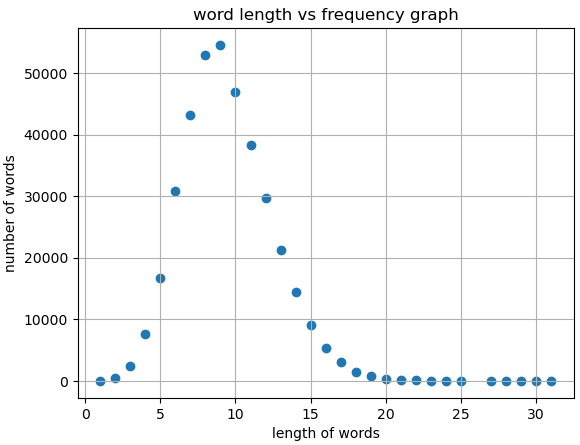
\includegraphics[width=0.5\textwidth]{./images/histogram.png}
\end{center}

We may notice that a large portion of available words are 5 to 10 characters long.

\subsection{Constructing a graph}

Using the words and based on the problem statement, we will attempt to construct a graph using the below algorithm.

\begin{lstlisting}[language=Python]
	def generate(word):
		yield from [
			word[:i] + '_' + word[i+1:]
			for i in range(len(word))
		]
	def construct_graph():
		graph = defaultdict(lambda : defaultdict(set))
		for length, words in self.word_map.items():
			for word in words:
				for i in range(len(word)):
					pattern = word[:i] + '_' + word[i+1:]
					graph[length][pattern].add(word)
		return graph
\end{lstlisting}

We attempt to create separate graphs for different word lengths, as the length of a word does not change throughout the problem. The obtained graph would look like the following (for a word `COOL`):

\begin{center}
	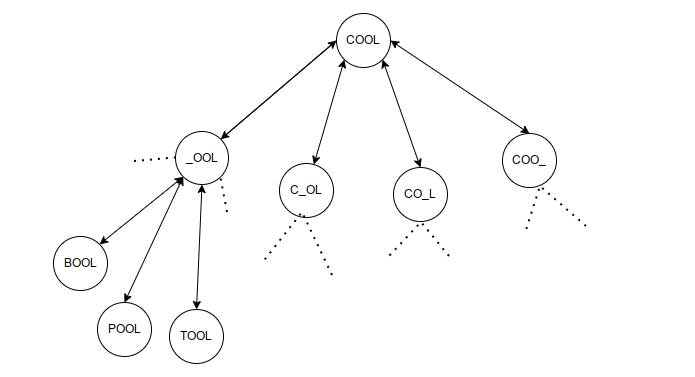
\includegraphics[width=0.5\textwidth]{./images/graph.png}	
\end{center}


Now, this graph can be traversed by using algorithms, and we can obtain a chain connecting two words on the graph. Construction of the graph can happen on the fly (while traversing), but due to the size of our corpus, we are constructing the graph before traversing to facilitate analysis. The constructed graph has over 50,00,000 nodes, a much higher number than the number of words in the corpus, as a large number of words get repeated.

\subsection{Traversing the graph}

Due to the number of nodes in the constructed graph, we may not use the depth-first search algorithm as the it would not be able to backtrack long paths. But a breadth-first search is applicable.

\begin{lstlisting}[language=Python]
	from collections import deque
	
	def bfs(begin, end, words, graph_):
		assert not {begin, end} - words
		assert len(begin) == len(end)
		graph = graph_[len(begin)]
		
		queue = deque([(begin, [begin])])
		visited = set([begin])
		
		iterations = 0
		while queue:
			w, path = queue.popleft()
			if w == end:  # goal
				return {"length": len(path), "iterations": iterations}
			for pattern in generate(w):
				delta = graph[pattern] - visited
				queue.extend([(d, path+[d]) for d in delta])
				visited.update(delta)
			iterations += 1
		
		return {"length": float('inf'), "iterations": iterations} # fail
\end{lstlisting}

Upon analysis, the above algorithm takes at least 1,000-10,000 iterations for traversing the graph (for word lengths more than 5) and gives an optimal solution. To minimize the number of iterations, we can use the bidirectional breadth-first search algorithm, where we maintain two queues and check for intersection between the visited sets.

\begin{lstlisting}[language=Python]
	def bfs_step(queue, visited, graph):
		q2 = deque()
		iterations = 0
		while queue:
			w, path = queue.popleft()
			for pattern in generate(w):
				delta = graph[pattern] - visited
				visited.update(delta)
				q2.extend([[nw, path + [nw]] for nw in delta])
			iterations += 1
		return q2, iterations
				
	def bi_bfs(begin, end, words, graph_):
		assert not {begin, end} - words
		assert len(begin) == len(end)
		graph = graph_[len(begin)]
	
		q1 = deque([[begin, [begin]]])
		q2 = deque([[end, [end]]])
	
		v1 = set([begin])
		v2 = set([end])
		
		iterations = 0
		while q1 and q2:
			if v1.intersection(v2): # goal
				_, path1 = q1.popleft()
				_, path2 = q2.popleft()
				path = path1 + path2[::-1]
				return {"length": len(path), 
					"iterations": iterations}
		
			if len(q1) <= len(q2):
				q1, it = bfs_step(q1, v1, graph)
			else:
				q2, it = bfs_step(q2, v2, graph)
			iterations += it
		
		return {"length": float('inf'), "iterations": iterations} # fail
\end{lstlisting}

The above algorithm does not exceed 500 iterations for finding a solution and returns an optimal solution comparable to the traditional breadth-first search algorithm. But, in order to guide the search, we can use the variants of A$\star$.

\subsection{Guided Search}

For using the variants of A$\star$, we need an admissible heuristic function. From analysis, the best heuristic function is found to be:

\begin{lstlisting}[language=Python]
	def heuristic(w, w2):
		return sum([a != b for a, b in zip(w, w2)])
\end{lstlisting}

The heurustic function is clearly the distance of word `w` from the word `w2`.

Using the above heuristic function, the following algorithm can be used to find a word ladder:

\begin{lstlisting}[language=Python]
	def astar(start, end, words, graph_, heuristic):
		assert not {start, end} - words
		assert len(start) == len(end)
		
		pq = [[heuristic(start, end), 0, start, [start]]]
		visited = set()
		graph = graph_[len(start)]
		
		iterations = 0
		while pq:
			_, cost, w, path = heapq.heappop(pq)
			if w == end: 
				return {"length": len(path), "iterations": iterations}
			for p in generate(w):
				delta = graph[p] - visited
				visited.update(delta)
				priorities = [cost + heuristic(w, end) for w in delta]
				pq.extend([(p, 1+cost, w, path + [w]) for w, p in zip(delta, priorities)])
			heapq.heapify(pq)
			iterations += 1
			
		return {"length": float('inf'), "iterations": iterations}	
\end{lstlisting}

This algorithm performs worse than the Bi-directional breadth-first search algorithm, as it traverses through many nodes which are away from the end word. To solve this problem, we can use the bi-directional A$\star$ algorithm. The following algorithm can be used to guide the search efficiently.

\begin{lstlisting}[language=Python]
	def bi_astar(start, end, words, graph_, heuristic):
		assert not {start, end} - words
		assert len(start) == len(end)
		
		graph = graph_[len(start)]
		
		pq1 = [(heuristic(start, end), 0, start, [start])]
		pq2 = [(heuristic(end, end), 0, end, [end])]
		
		v1, v2 = set(), set()
		iterations = 0
		
		while pq1 and pq2:
			if v1.intersection(v2):
				*_, path1 = pq1[0]
				*_, path2 = pq2[0]
				path = path1 + path2[::-1]
				return {"length": len(path), "iterations": iterations}
		
			it = 0
		
			if len(pq1) <= len(pq2):
				pq1_ = []
				while pq1:
					it += 1
					_, c1, w1, path1 = heapq.heappop(pq1)
					
					for p in generate(w1):  
						delta = graph[p] - v1
						v1.update(delta)
						priorities = [c1 + heuristic(w, end) for w in delta]
						pq1_.extend([(p, 1+c1, w, path1 + [w]) for w, p in zip(delta, priorities)])
					pq1 = pq1_
					heapq.heapify(pq1)
			
			else:
				pq2_ = []
				while pq2:
					it += 1
					_, c2, w2, path2 = heapq.heappop(pq2)
					
					for p in generate(w2):
						delta = graph[p] - v2
						v2.update(delta)
						priorities = [c2 + heuristic(w, end) for w in delta]
						pq2_.extend([(p, 1+c2, w, path2 + [w]) for w, p in zip(delta, priorities)])
				pq2 = pq2_
				heapq.heapify(pq2)
				
			iterations += it
		return {"length": float('inf'), "iterations": iterations}
\end{lstlisting}

The above algorithm performs on-par with the bi-directional breadth first algorithm. The following graph compares all the above algorithms in terms of number of iterations taken.

\begin{center}
	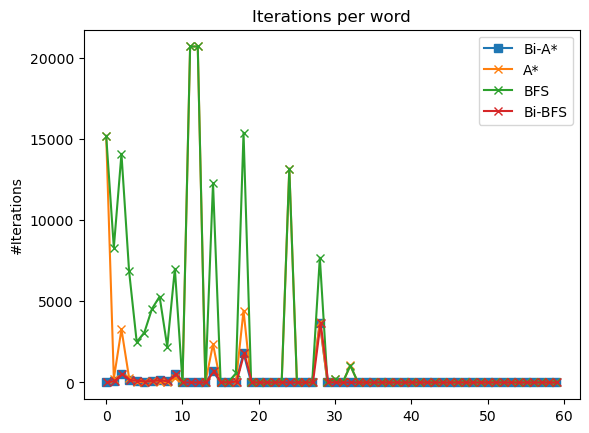
\includegraphics[width=0.6\textwidth]{images/iterations-index.png}
\end{center}

The following plot shows the length of the word chain found through various algorithms:

\begin{center}
	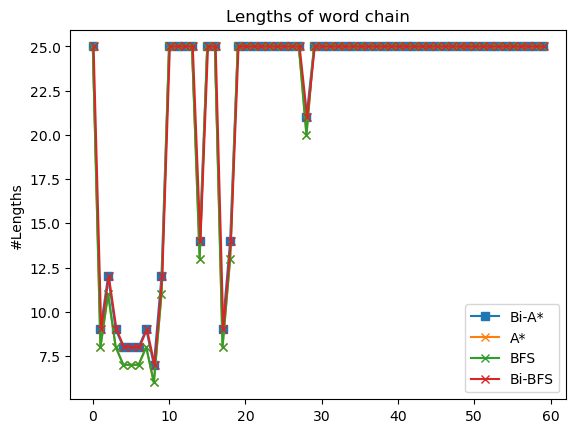
\includegraphics[width=0.6\textwidth]{images/lengths.png}
\end{center}

The above plot shows that the BFS algorithm performs better than other algorithms in terms of the length of the word chain, but takes a large number of iterations.

\section{Conclusion}

In conclusion, the word ladder problem is explored using 4 different algorithms, and it can be seen that BFS algorithm produces shorter chains than the guided-search algorithms.

\end{document}
